\documentclass{article}
\usepackage{amsmath}
\usepackage[utf8]{inputenc}
\usepackage{float}
\usepackage{epsfig,graphicx}
\usepackage{xcolor,import}
\usepackage[german]{babel}
\usepackage{textcomp}
\usepackage{mathtools}

\begin{document}
\thispagestyle{empty}
			\begin{center}
			\Large{Fakultät für Physik}\\
			\end{center}
\begin{verbatim}


\end{verbatim}
							%Eintrag des Wintersemesters
			\begin{center}
			\textbf{\LARGE WINTERSEMESTER 2014/15}
			\end{center}
\begin{verbatim}


\end{verbatim}
			\begin{center}
			\textbf{\LARGE{Physikalisches Praktikum 1}}
			\end{center}
\begin{verbatim}




\end{verbatim}

			\begin{center}
			\textbf{\LARGE{PROTOKOLL}}
			\end{center}
			
\begin{verbatim}





\end{verbatim}

			\begin{flushleft}
			\textbf{\Large{Experiment (Nr., Titel):}}\\
							%Experiment Nr. und Titel statt den Punkten eintragen
			\LARGE{3. Elastizität / Trägheitsmoment}	
			\end{flushleft}

\begin{verbatim}

\end{verbatim}	
							%Eintragen des Abgabedatums, oder des Erstelldatums des Protokolls
			\begin{flushleft}
			\textbf{\Large{Datum:}} \Large{31.10.2014}
			\end{flushleft}
			
\begin{verbatim}
\end{verbatim}
							%Namen der Protokollschreiber
		\begin{flushleft}
			\textbf{\Large{Namen:}} \Large{Veronika Bachleitner, Erik Grafendorfer}
			\end{flushleft}

\begin{verbatim}


\end{verbatim}
							%Kurstag und Gruppennummer, zb. Fr/5
			\begin{flushleft}
			\textbf{\Large{Kurstag/Gruppe:}} \Large{Fr/1}
			\end{flushleft}

\begin{verbatim}






\end{verbatim}
							%Name des Betreuers, das Praktikum betreute.
			\begin{flushleft}
			\LARGE{\textbf{Betreuer:}}	\Large{SETMAN}	
			\end{flushleft}
			
\newpage
\section{Spannungs-Dehnungs-Kurve von Aluminium}
\subsection{Aufgabenstellung}
Wir messen erst die Dicke eines Aluminiumdrahtes, dann spannen wir ihn zwischen die Balken eines Materialprüfgerätes, dehnen ihn in gleichen Zeitabschnitten gleiche kleine Längen und messen mit einem von uns kalibrierten Messverstärker die Kraft, die auf ihn wirkt. Aus der Kraft und der Dicke des Drahtes berechnen wir die Spannung, die auf ihn wirkt, vergleichen sie mit der Dehnung, die er erfuhr. Wir bestimmen so das Verhältnis der Spannung und der Dehnung des Drahtes, den E-Modul und versuchen seine Streckgrenze auf verschiedene Arten zu ermitteln.
\subsection{Grundlagen}
Wenn Kräfte auf Festkörper wirken, gibt es zwei physikalisch völlig unterschiedliche Arten der Verformung, die sie erleiden: Die \textit{elastische} und die \textit{plastische} Verformung. Die elastische Verformung basiert auf Kräften zwischen den Atomen selbst, während die plastische auf Deformierungen im Kristallgitter des Körpers beruht. \\
\\Die Spannung $\sigma$ auf einen Körper ist die auf ihn wirkende Kraft pro der Fläche, auf der sie wirkt:  $$ \sigma = \frac{F}{A} $$ \\
Die Dehnung  $\varepsilon$ ist das Verhältnis aus der Längenänderung $\Delta$l und seiner ganzen Länge l, die der Körper bei der Dehnug erfährt: \\
$$ \varepsilon= \frac{\Delta l}{l} $$ \\
 Wir überlegen: Während einer elastischen Verformung des Drahtes bleibt das Verhältnis von Spannung und Dehnung annähernd konstant, weil es keine qualitativen Änderungen in seiner Struktur gibt - darum kehrt ein Körper nach einer elastischen Verformung auch in seinen Ausgangszustand zurück. Beginnt allerdings die plastische Verformung, gibt es kein zurück - die Kristallstruktur des armen Körpers wird dauerhaft verändert, seine Dehnung fällt leichter weil seine Integrität zerstört wird. Wir wollen den Übergang von elastischer zu plastischer Verformung genau ermitteln, indem wir die Spannung $\sigma$ pro Dehnung $\varepsilon$ darstellen und untersuchen, wo das Verhältnis konstant ist und wo plötzlich mehr Dehnung bei gleich anwachsender Spannung gemessen wird. Den Quotienten aus der Spannung und der Dehnung nennt man den \textit{E-Modul E}:

$$ E=\frac{\sigma}{\varepsilon}$$

Die Streckgrenze markiert den Übergang von der elastischen zur plastischen Verformung. Für sie brauchen wir auch die elastische Gerade, die durch den Bereich gefittet wird, in dem die Spannung linear mit der Dehnung ansteigt. Wir beschreiben vier Varianten der Streckgrenze:
\begin{enumerate}
\item \textbf{Elastizitätsgrenze} Erste sichtbare Abweichung von der elastischen Gerade.
\item \textbf{0.05\%-Streckgrenze} Um $\Delta \varepsilon$=0.05\% parallelverschobene Gerade, geschnitten mit der Kurve.
\item \textbf{0.2\%-Streckgrenze} Analog mit 0.2\%.
\item \textbf{Rückextrapolierte Streckgrenze} Wir schneiden die elastische Gerade mit einer Geraden, die im plastischen Bereich gefittet wird, sofern der plastische Bereich wieder linear verläuft.
\end{enumerate}

Einheiten der Größen:
$$[\sigma]=\frac{N}{m^2}$$
$$[E]=\frac{N}{m^2}$$
\subsection{Versuchsaufbau und Methoden}
Wir verwenden Prüfmaschine der Fa. INSTRON zur Dehnung des Drahts. Diese Maschine besitzt einen Ausgang, der eine Spannung relativ zur auf den Draht gemessenen Kraft ausgibt und mittels eines Messverstärkers verstärkt wird. Dieses Signal wird dann mittels eines Analog/Digitalwandlers der Firma National Instruments an den Messcomputer gesendet. Parallel zum Analogausgang des Verstärkers wird ein Voltmeter zur Kalibrierung des Messverstärkers geschalten.
Wir erhalten $\sigma$ durch Division der gemessenen Kraft durch den gemessenen Probenquerschnitt q:
$$ \sigma = \frac{F}{q}$$
$\varepsilon$ ist das Verhältnis der Längenänderung, die die Maschine verursacht, v$\cdot$t, zur ursprünglichen Einspannlänge der Probe.
$$ \varepsilon = \frac{v\cdot t}{L_0} \text{hier} = \frac{0.5\frac{mm}{min}}{100mm} = \frac{8.\bar{3}\cdot10^{-3}\frac{mm}{s}}{100mm}$$
\subsection{Durchführung}
Wir schalten den alten Röhrenverstärker an und lassen ihn aufwärmen. Währenddessen führen wir das andere Experiment in unserer Serie durch, das Torsionspendel. Dann beginnen wir mit diesem Experiment: \\
Wir kalibrieren den Verstärker indem wir per BALANCE regeln, bis unser angeschlossenes Voltmeter 0V anzeigt. Dann hängen wir 2kg an die Materialprüfmaschine und regeln per CALIBRATION, bis unser Messgerät 0.040V anzeigt.
Wir messen den Durchmesser des Drahtes fünf Mal und bilden einen Mittelwert. Wir spannen ihn ein und verbiegen ihn sehr stark, weil wir mit zu viel maskuliner Kraft rangegangen sind. Also nehmen wir einen neuen Draht, messen seinen Durchmesser und spannen ihn diesmal vorsichtiger ein. Dann dehnen wir den Draht gleichmäßig, während wir die dafür notwendige Kraft mit dem analogen Messverstärker messen und das Signal über einen Analog/Digitalwandler in einen Computer schicken und es dort mit einer dafür von der Universität zur Verfügung gestellten Software 'Zugversuch' aufzeichnen, um es später mit qtiplot zu analysieren.
\subsection{Ergebnisse}

\subsubsection*{Querschnitt des Drahtes}
$$\bar{q}=(2.00 \pm 0.05)mm$$ 
\subsubsection*{Zugversuch}
\begin{center}
\begin{figure}
\caption{Elektrische Spannung zu Zeit}
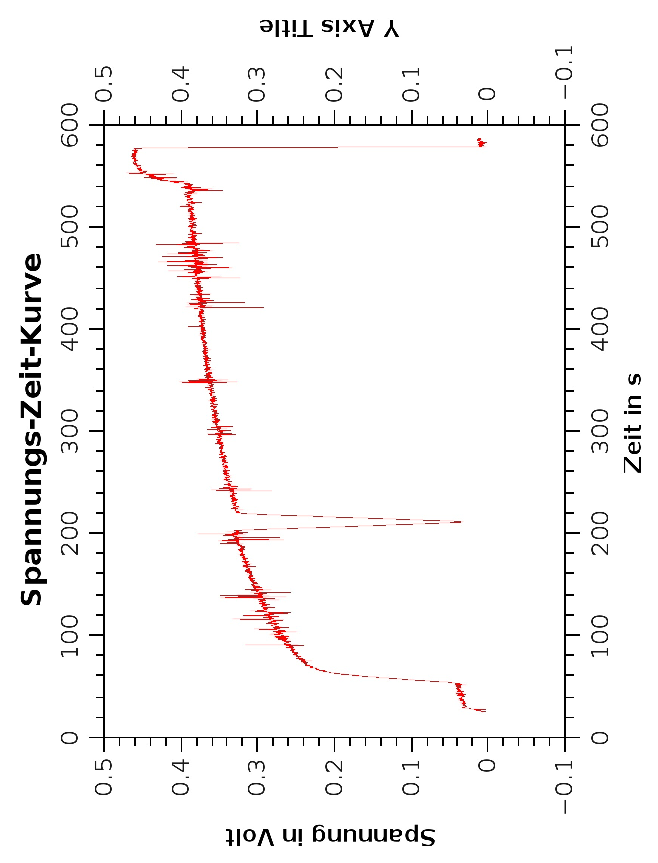
\includegraphics[scale=0.8, angle=-90]{voltzeitkurve.eps}
\end{figure}
\end{center}
\begin{center}
\begin{figure}
\caption{Kraft zu Zeit}
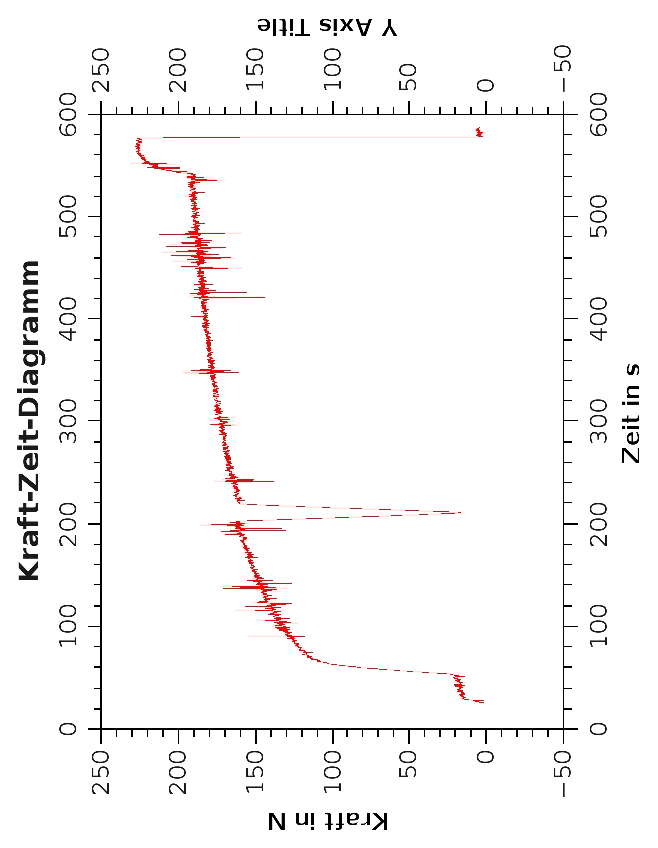
\includegraphics[scale=0.8, angle=-90]{kraftzeitkurve.eps}
\end{figure}
\end{center}
Die Steigung der gefitteten Gerade durch unseren ersten Andehnversuch: 
$$ (41.15 \pm 487) \frac{kN}{mm^2} od. GPa $$

Die Steigung der gefitteten Gerade durch unseren zweiten Andehnversuch:
$$ (17.79 \pm 151) \frac{kN}{mm^2} od. GPa $$

\begin{center}
\begin{figure}
\caption{Mechanische Spannung zu relativer Dehnung}
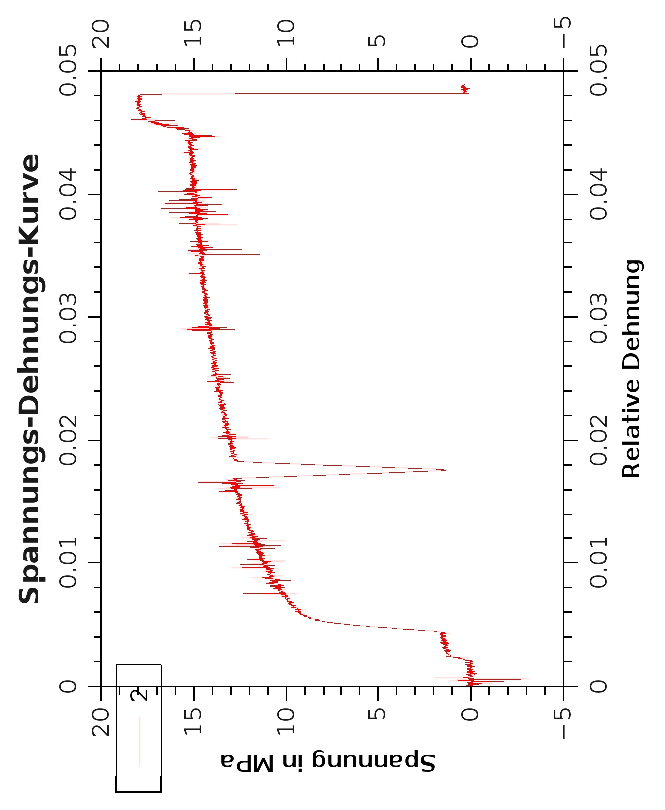
\includegraphics[scale=0.7,angle=-90]{spannungsdehnungskurve.eps}
\end{figure}
\end{center}
\subsubsection*{Bestimmung des E-Moduls}
\subsubsection*{Bestimmung der Streckgrenze}
\subsection{Diskussion}
\newpage
=======
Uns fällt auf dass sogar unser zweiter, gemessener Wert stark des E-Moduls weit unter dem
Literaturwert zum E-Modul von Aluminum von 70 kN/mm² [Tipler] liegt. Wir müssen daher leider davon ausgehen, dass wir schlecht gemessen haben. Womöglich hat sich unser zweiter, femininerer Einspannversuch doch als zu schwach erwiesen, wodurch der Draht rutschen konnte - oder vielleicht ist doch, etwas aufgeklärter, die Halterung des alten Geräts schon locker.

\section{Bestimmung des Schubmoduls von Aluminium mit dem Torsionspendel}
\subsection{Aufgabenstellung}
Wir befestigen zwei Gewichte an den Enden einer Querstange, hängen diese an ihrer Mitte an einen Aluminiumdraht und versetzen die Stange ihn Rotation. Aus ihrer Schwingungsdauer berechnen wir dann das Schubmodul, auch Torsionsmodul genannt, des Aluminiumdrahts.
\subsection{Grundlagen}
Die Schubspannung $\tau$= F/A ist proportional zum Tangens des Scherwinkels $\alpha$:
$$ \tau = G\cdot	tan\alpha$$

Abhängig von der Drehung der Stange $\phi$ entsteht ein rückstellendes Moment M durch die Torsion des Drahtes:
$$M=-D\phi$$
D ist das Direktionsmoment. Lässt man die Querstange los, schwingt sie mit der Periodendauer T:
$$T=2\pi \sqrt{\frac{J}{D}}$$
wobei J das Trägheitsmoment der gesamten Anordnung ist. Wenn sich die Stange dreht, wird der Draht geschert, und nachdem Scherungen durch das Schubmodul beschrieben werden können, steht das Direktionsmoment in einem Zusammenhang mit dem Schubmodul G:
\begin{equation} 
\label{G}
G = \frac{2LD}{\pi r^4}
\end{equation}
r ist der Radius des Drahtes, L seine Länge. \\
Man verwendet ein Differenzverfahren um J zu bestimmen. $J_A$ sei das Trägheitsmoment ohne Zusatzgewichte, $J_Z$ mit Gewichten. Mit dem Satz von Steiner lässt sich $J_Z$ zu dem Trägheitsmoment bezüglich der Rotation um eine Schwerpunktachse, $J_S$, + m$l^2$ vereinfachen:
\begin{equation} \label{J}
J =  J_A + 2\cdot J_Z = J_A + 2 \cdot (J_S + ml^2)
\end{equation} 
Misst man nun die Periodendauern $T_1$,$T_2$ für zwei verschiedene Distanzen $l_1$,$l_2$ der Zusatzgewichte, so kann man die unbekannten Größen $J_A$ und $J_Z$ eliminieren. Dazu quadriert man die beiden Ausdrücke für $T_1$ und $T_2$ und substrahiert sie voneinander: 
$$T_1^2-T_2^2 = 8 \pi^2m\frac{l_1^2-l_2^2}{D}$$
Dies formt man nach D um und setzt in  \ref{G} ein:
\begin{equation}
\label{Gfinal}
G=16\pi\frac{LM(l_1^2-l_2^2)}{r^4(T_1^2-T_2^2)}
\end{equation} 
Wir berechnen auch die Poissonzahl $\nu$, das Verhältnis der relativen Querkontraktion $\Delta d / d$, die bei der Verformung des Drahtes geschieht, und der relativen Längenänderung $\Delta l$ /l.
$$\nu=\frac{\Delta d / d}{\Delta l / l} $$

Zwischen E,G und $nu$ besteht eine Beziehung für linear elastische, isotrope Materialien:

$$\nu = \frac{E}{2G} -1$$
Für diesen Abschnitt wurde auf die Aufgabenstellung zurückgegriffen.
\subsection{Versuchsaufbau und Methoden}
Wir befestigen eine Querstange, an deren Enden zwei Gewichte hängen, an einem Aluminiumdraht. Wir messen die Dicke des Drahtes, die Massen der Gewichte und setzen die Querstange in Rotation. Schließlich messen wir ihre Schwingungsdauern 10 mal in Folge, und das 10 mal. \\
Wir messen die Dauer mit einer Stoppuhr, die wir händisch auslösen. Die Auslenkung aus der Ruhelage der Querstange beträgt etwa 10°. \\
Wir verwenden zwei verschieden schwere Gewichtpaare die auf verschiedenen Längen der Querstange montiert sind.
\subsection{Ergebnisse}
\subsubsection*{Dicke des Drahtes}
$$\bar{q}=(3.15 \pm 0.05)mm$$ 
\subsubsection*{Massen der Gewichte}
$$m_1=(349.5 \pm 0.5)g$$
$$m_2=(230.5 \pm 0.5)g$$
$$m_{mount}=(17.0 \pm 0.5)g$$\\
Wobei $m_{mount}$ die Masse der Aufhängung für die Gewichte ist. Daher ist die tatsächliche Masse:
$$M_1=m_1+m_{mount}=(366.5 \pm 0.5)g$$
$$M_2=m_2+m_{mount}=(247.5 \pm 0.5)g$$
\subsubsection*{Abstand der Gewichte}
\begin{gather*}
l_{1a}=(200 \pm 1)mm\\
l_{1b}=(130 \pm 1)mm\\
l_{2a}=(170 \pm 1)mm\\
l_{2b}=(70 \pm 1)mm
\end{gather*}
Außerdem die Länge des Pendels: L=$(627 \pm 1)mm$
\subsubsection*{Schwingungsdauern}
\begin{gather*}
\bar{T_{1a}}=(1.99 \pm 0.03)s\\
\bar{T_{1b}}=(1.45 \pm 0.05)s\\
\bar{T_{2a}}=(1.46 \pm 0.03)s\\
\bar{T_{2b}}=(0.99 \pm 0.08)s
\end{gather*}
Wobei es sich bei den Unsicherheiten um die Standardabweichungen der Mittelwerte handelt, die mit dem Taschenrechner berechnet wurden.
\subsubsection*{Schubmodul}
\begin{gather*}
G_1=16\pi\frac{LM_1(l_{1a}^2-l_{1b}^2)}{r^4(T_{1a}^2-T_{1b}^2)}=2.334*10^{10} Pa\\
G_2=16\pi\frac{LM_2(l_{2a}^2-l_{2b}^2)}{r^4(T_{2a}^2-T_{2b}^2)}=2.642*10^{10} Pa
\end{gather*} 
\subsubsection*{Fehlerrechnung zum Schubmodul:}
Wir berechnen für $G_1$ sowie für $G_2$ unter Berücksichtigung der Unsicherheiten aller Werte den Größtfehler:
\begin{gather*}
G^{min}_1=2.204*10^{10} Pa\\
G^{max}_1=2.479*10^{10} Pa\\
G^{min}_2=2.625*10^{10} Pa\\
G^{max}_2=2.697*10^{10} Pa
\end{gather*}
Daraus ergeben sich die Unsicherheiten: $Delta_1=1.38$ und $Delta_2=0.36$
Da wir zwei Messungen mit verschiedenen Einstellungen haben, wollen wir aus beiden das gewogene Mittel:
\begin{gather*}
\delta_1=1/(1.38)^2=0.525\\
\delta_2=1/(0.36)^2=7.716\\
G_{gewichtet}=\frac{G_1*\delta_1 + G_2*\delta_2}{\delta_1 + \delta_2}=26.22 GPa\\
\Delta G_{gewichtet}=\sqrt{\frac{0.525(23.34-26.22)^2+7.716(26.42-26.22)^2}{(2-1)*(0.525+7.716)}}=0.753
\end{gather*}
Daraus ergibt sich unser Endergebnis für das Schubmodul:\\
$$\boxed{(G=26.22 \pm 0.76) GPa}$$\\
\\
Da unser Ergebnis für das Elastizitätsmodul aus dem ersten Experiment nicht den Literaturwerten entspricht, verwenden wir hier für die Berechnung der Poissonzahl den Literaturwert für E: $E=70GPa$\\
Damit ist die Poissonzahl:\\
$$\nu = \frac{E}{2G} -1  = \frac{70}{2*26.22} -1\\$$\\
$$\boxed{\nu = 0.335 \pm 0.039}$$
\subsection{Diskussion}
Beim Berechnen der Werte ist immer sorgfältig darauf zu achten, die Größen mit den richtigen Einheiten einzusetzen.\\
Das aus unserer Messung errechnete Schubmodul beträgt:\\
$(G=26.22 \pm 0.76) GPa$\\
Literaturwert [Wikipedia] zum Schubmodul von Aluminium: $25.5 kN/mm^2 = 25.5 GPa$\\
Da dieser Wert in Ordnung ist und wir für das Elastizitätsmodul den Literaturwert verwendet haben, bekommen wir natürlich auch für die Poissonzahl ein gutes Ergebnis: $\nu = 0.335 \pm 0.039$\\
Literaturwert [Wikipedia] zur Poissonzahl von Aluminium: 0.34\\
Wir sind mit dieser Messung also zufrieden und wollen uns in Hinblick auf die Fehlerrechnung auch bei Captain Kirk  bedanken, der uns unermüdlich unterstützt hat.\footnote{Vergleiche Youtube: Captain Kirk is Climbing a Mountain (4 Hour Version)}
\newpage
\section{Physikalisches Pendel}
\subsection{Aufgabenstellung}
Wir führen Messungen mit einem Fahrradpendel durch. Dazu messen wir die Schwingungsdauer in Abhängigkeit des Auslenkwinkels über einen Bereich von 10° bis 100° dar und verarbeiten und diskutieren anschließend unsere Messwerte. 
Daraus berechnen wir uns auch weitere Ergebnisse wie die Winkelrichtgröße des Pendels und die Trägheitsmomente von Pendel, Zusatzmasse und Rad. 

\subsection{Grundlagen}
Auslenkwinkel $\phi(t)$: [$\phi(t)$]=1(rad)\\
Zeit t: $[t]=s$\\
Masse m: $[m]=kg$\\
Länge l: $[l]=m$\\
Periodendauer T: $[T]=s$\\
Winkelbeschleunigung $\ddot{\phi}$: [$\ddot{\phi}$]=$s^{-2}$\\
Winkelrichtgröße D: $[D]=kg \frac{m^2}{s^2}$\\
Erdbeschleunigung: $g=9.81ms^{-2}$\\
\\
\textbf{Mathematisches Pendel}\\
Ein mathematische Pendel ist ein idealisiertes Objekt und besteht aus einem masselosen Faden und einer im Schwerpunkt konzentrierten Masse. Reibungs- und Strömungswiderstände werden vernachlässigt, sodass eine konstante Schwingungsdauer $T_0$ angenommen werden kann.\\
\\
Bewegungsgleichung:
\begin{equation*}
\ddot{\phi}(t)+\frac{g}{l}sin(\phi(t))=0
\end{equation*}\\
Lösung für kleine Winkel:
\begin{equation*}
\phi(t)=\phi_0cos(\sqrt{\frac{g}{l}}t+\Phi)
\end{equation*}
wobei $\phi_0$ der maximale Auslenkungswinkel und $\Phi$ die Anfangsphase bei t=0 ist. \\
\\
Periodendauer:
\begin{equation*}
T_0 = \frac{2\pi}{\omega} = 2\pi\sqrt{\frac{l}{g}}
\end{equation*}\\
\\
\textbf{Physikalisches Pendel}\\
Im Gegensatz zum mathematischen Pendel, schwingt beim physikalischen Pendel ein Körper um eine Achse, die \textit{nicht} durch den Schwerpunkt verläuft.\\
Die Bewegungsgleichung muss jetzt anders bestimmt werden:
\begin{equation*}
J\ddot{\phi(t)} + D sin(\phi(t)) = 0
\end{equation*}
wobei die Winkelrichtgröße $D=mgl$\\
\\
Schwingungsdauer: $T_0=\frac{2\pi}{\omega}=2\pi\sqrt{\frac{J}{D}}$\\
\\
Steiner'scher Satz: $J = J_S + m_{ges} d^2$\\
wobei $J_S$ das Trägheitsmoment bezüglich einer Achse um den Schwerpunkt, J das Trägheitsmoment bezüglich einer parallelen Achse im Abstand d.\\
\\
\textbf{Fahrradpendel}\\
Ein in Wirklichkeit realisiertes Pendel kann folgendermaßen aussehen:
%\includegraphics[scale=0.1,angle=-90]{fahrradpendel.eps}
Wir sehen hier, dass es sich um ein Speichenrad mit zylindrischer Zusatzmasse handelt.\\
\\
Winkelrichtgröße:
$$D=m_Z g l_{AS}$$
wobei $l_{AS}=R_F + \frac{h_Z}{2}$, $R_F$ der Radius der Felge, $h_Z$ die Höhe der Zusatzmasse.\\
\\
Trägheitsmoment:
\begin{equation*}
J = J_Z + J_{Rad} = D (\frac{T_0}{2\pi})^2
\end{equation*}
\\
wobei das Trägheitsmoment des Zylinders:
\begin{equation*}
J_Z = m_Z(\frac{1}{4}r^2_Z + \frac{1}{12}h^2_Z+l^2_{AS})
\end{equation*}
\\
Das Trägheitsmoment des Rades wird rückschließend bestimmt durch Nutzung der Gleichung für das gesamte Trägeheitsmoment.
\\
\subsection{Ergebnisse}
\textbf{Schwingungsdauer T}\\
\\
\begin{tabular}{ r | l }
Winkel & Zeit \\ \hline
100.0 & 1.853\\
90.0	 & 1.772\\
80.0	 & 1.705\\
70.0	 & 1.648\\
60.0	 & 1.603\\
50.0 & 1.566\\
40.0	 & 1.536\\
30.0	 & 1.513\\
20.0	 & 1.498\\
10.0	 & 1.486\\
\end{tabular}
\\
\\
T als Funktion von $\phi_0$, Polynomfit mit $a_0+a_1x^2+a_2x^4$: \\
%GRAPH!
\\
Die Unsicherheiten wurden dem Anleitungstext entnommen.\\
QTI-Plot ist so zuvorkommend und gibt uns folgende Daten:
\begin{quote}
Scaled Levenberg-Marquardt algorithm with tolerance = 0.0001\\
From $x = 1.0000000000000*10^{01}$ to $x = 1.0000000000000*10^{02}$\\
$a_0 = 1.4849559932346  \pm 7.2819000012540*10^{04}$\\
$a_1 = 3.0370131473218*10^{05} \pm 4.0483211759158*10^{07}$\\
$a_2 = 6.3628471138547*10^{10} \pm 4.0785013174204*10^{11}$
\end{quote}
Daraus lesen wir ab, dass die Schwingungsdauer für sehr kleine Auslenkungen:\\  $$\boxed{T_0=a_0=(1.48496 \pm 0.00073)s}$$\\
\\
\textbf{Winkelrichtgröße}\\
\begin{gather*}
m_Z=(938.5 \pm 0.1)g\\
l_{AS}=(388 \pm 1)mm\\
D=m_Zgl_{AS}=0.9385 * 9.81 * 0.388 = \boxed{D=(3.5722 \pm 0.0096)J}
\end{gather*}
\\
\textbf{Trägheitsmoment des Pendels}\\
\begin{equation*}
J = J_Z + J_{Rad} = D (\frac{T_0}{2\pi})^2=\boxed{J=(0.1995 \pm 0.0074) kg m^2}\\
\end{equation*}
\\
\textbf{Trägheitsmoment der Zusatzmasse}\\
\begin{gather*}
r_Z=(35.28 \pm 0.02)mm\\
h_Z=(107.60 \pm 0.02)mm\\
J_Z = m_Z(\frac{1}{4}r^2_Z + \frac{1}{12}h^2_Z+l^2_{AS})=\boxed{J_Z=(0.1425 \pm 0.0075)kg m^2}\\
\end{gather*}
\\
\textbf{Trägheitsmoment des Rades}\\
$$\boxed{J_{Rad} = J - J_Z = (0.057 \pm 0.015)kg m^2}$$\\
\\
\subsection{Diskussion}
Der Umgang mit CASSY-Lab2 fiel uns nicht schwer, da die Anweisungen im Anleitungstext leicht zu befolgen waren.\\
Bei diesem Experiment haben wir allerdings unseren ersten Fehler während des Praktikums begangen: Vergessen, einige Größen zu messen. \\
Wir beziehen unsere Daten für $l_{AS}$, $r_Z$ und $h_Z$ daher mit freundlicher Genehmigung aus dem Protokoll von Johannes Kurz, Patrick Braun aus dem WS 2013/14 und hoffen, dass der Experiment-Aufbau sich seither nicht verändert hat. Die weiteren Berechnungen führen wir natürlich selbst durch. \\
Der Polynomfit 4. Ordnung passt sehr gut zu unseren Ergebnissen. Wir sehen dabei kaum Abweichung der gefitteten Kurve von den Messdaten.\\

\end{document}